
\subsection{Accuracy Metrics}
The fidelity of a compression can be measured by different accuracy metrics. This is done by calculating the distance between each point in the original trajectory and the new trajectory. From these distances, various operations can be performed to obtain an overall metric. The mean distance of all points is the most commonly used measure, but other metrics such as median or maximum can also provide valuable insights into accuracy. The method used to calculate the distance, determines the accuracy metric. Example distances are shown in figure \ref{fig:sed}. The following sections will explore the most used accuracy metrics, as menioned by, \cite{TrajFramework} and \cite{Sun2016}.

\subsubsection{Perpendicular Distance}
\label{foobar:PD}
Perpendicular distance (PD) refers to the shortest distance from a removed point to the new trajectory, as shown in figure \ref{fig:sed}. The shortest distance is always perpendicular to the trajectory, hence the name.

\subsubsection{Synchronized Euclidean Distance}
\label{subsub:SED}
SED is a measurement where a point $p_{i}$ is assigned a distance to the new trajectory that is equal to the distance to the synchronized point $p'_{i}$, as shown in figure \ref{fig:sed} $p'_{i}$ is calcluated as:
\begin{equation}
    \begin{aligned}
        t'_{i} & = t_{i}                                                \\
        x'_{i} & = x_{s} + \frac{t_{i}-t_{s}}{t_{e}-t_{s}}(x_{e}-x_{s}) \\
        y'_{i} & = y_{s} + \frac{t_{i}-t_{s}}{t_{e}-t_{s}}(y_{e}-y_{s}) \\
    \end{aligned}
\end{equation}
This error metric takes time into account. Two trajectories traversing the exact same spatial points might still be considered different if one took a longer time. This can be a useful metric for differentiating between taxi trips in rush hour and outside rush hour, since the trips outside rush hour will typically be shorter in duration.

\begin{figure}[ht]
    \begin{minipage}[b]{0.5\linewidth}
        \centering
        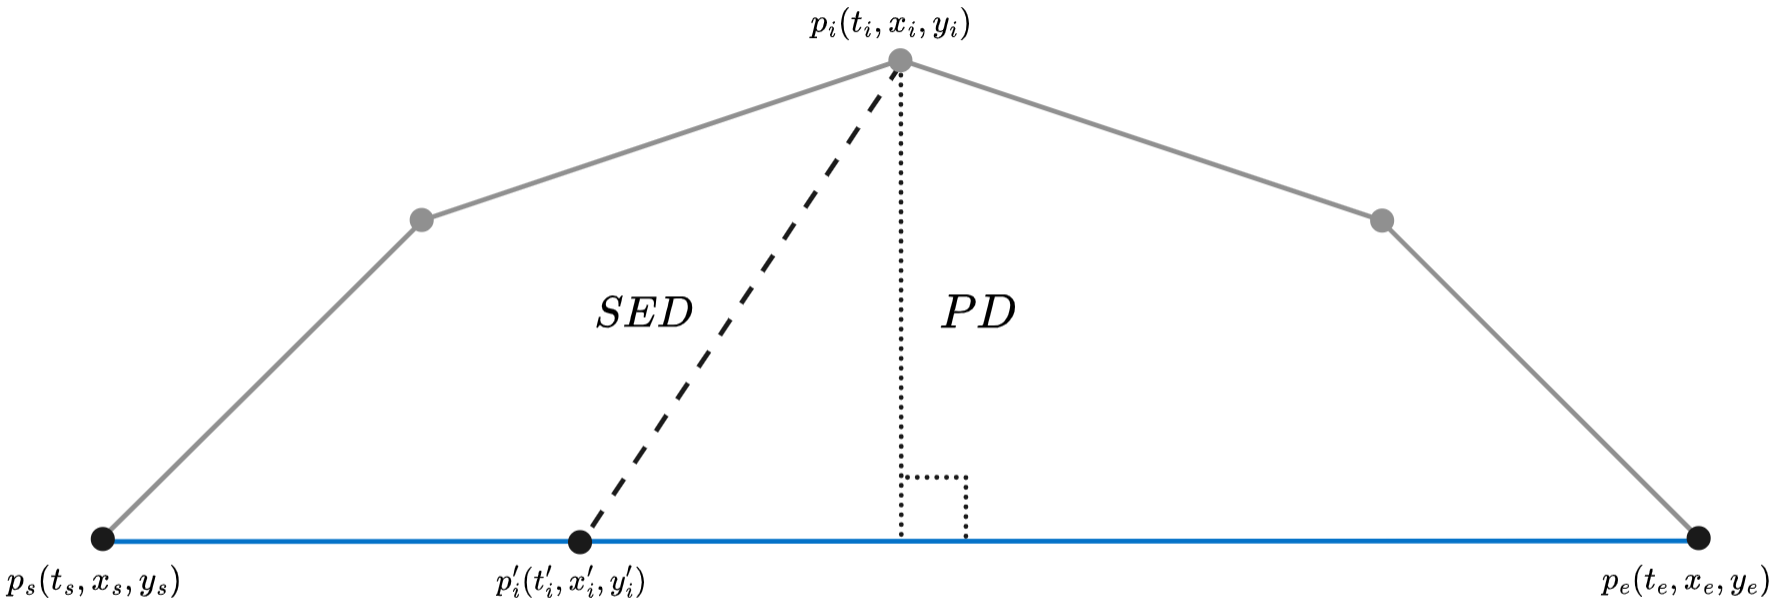
\includegraphics[width=\linewidth, height=7cm, keepaspectratio]{./figures/sed.png}
        \caption{Original trajectory in gray and new trajectory in blue showing distances SED and PD.}
        \label{fig:sed}
    \end{minipage}
    \begin{minipage}[b]{0.5\linewidth}
        \centering
        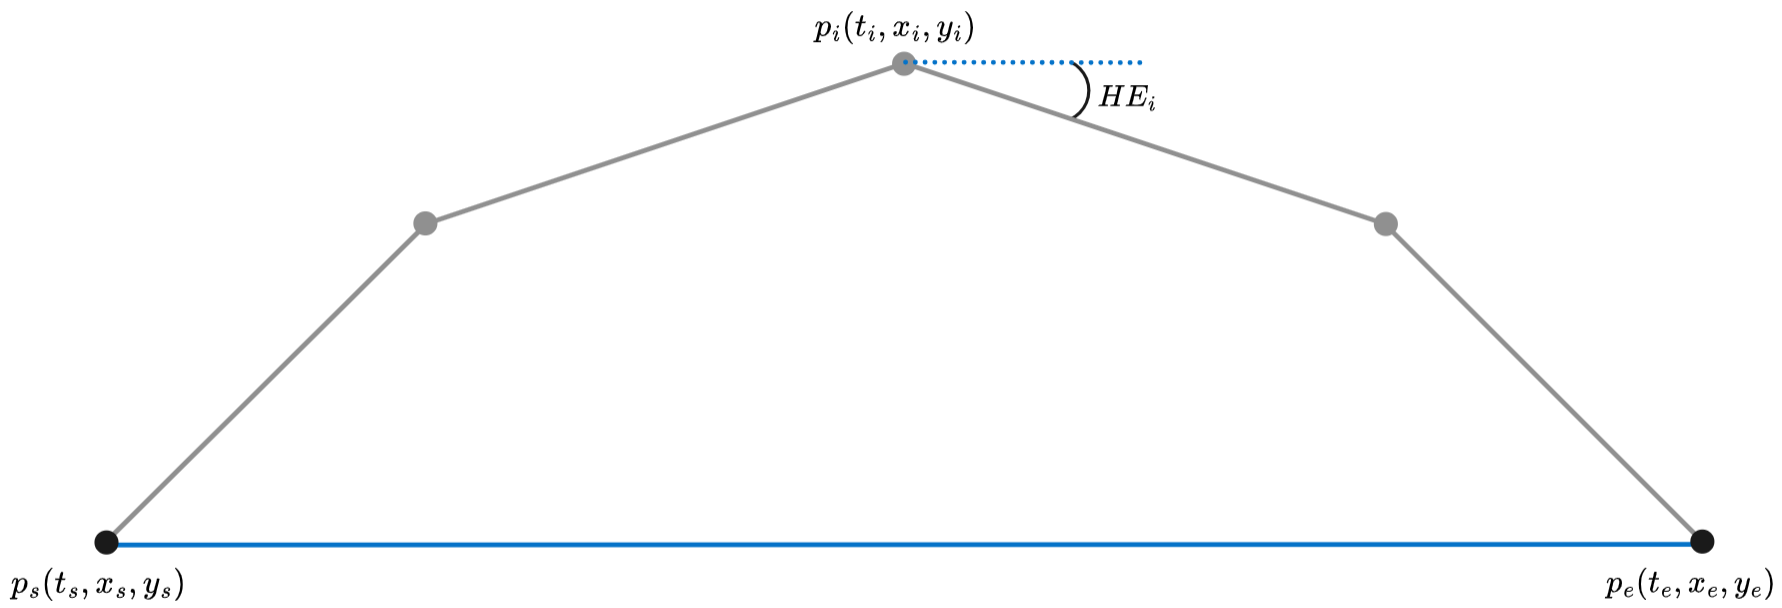
\includegraphics[width=\linewidth, height=7cm, keepaspectratio]{./figures/heading_error.png}
        \caption{Original trajectory in gray and new trajectory in blue showing distances HE.}
        \label{fig:hed}
    \end{minipage}
\end{figure}

\subsubsection{Heading Error}
The Heading Error (HE) for a point $p_{i}$ is the angular difference between the line segment $p_{i}$-$p_{i+1}$ along the original trajectory and $p'_{i}$-$p'_{i+1}$ along the compressed trajectory shown in figure \ref{fig:hed}. The angle represents the difference in direction between the original and the compressed trajectory at a given point. This metric is useful for detecting erratic movement and disruption of traffic flow according to \cite{TrajFramework}.

\subsubsection{Speed Error}
The Speed Error is similar to the Heading Error in that it compares the segments from the original trajectory with the corresponding segment in the compressed trajectory. However, it compares speed instead of direction. The Speed Error is the difference in speed between the original and compressed trajectory at a given point.

\subsubsection{Dynamic Time Warping}
Dynamic Time Warping (DTW) is an algorithm used to determine the alignment cost between two time series. It can align the series by finding which points correspond to each other and the distortion between corresponding points. The total alignment cost describes how similar the series are according to the DTW measure. When trying to align two very different series, the alignment cost will be high, for two similar series, it will be low. With regards to trajectory compression, the alignment cost between a compressed trajectory and the original describes how similar they are, or how much information is preserved in compressed form. A compression with high fidelity will have a low alignment cost.

The DTW algorithm works by calculating the distance matrix between two series. The distance $d_{i,j}$ in a matrix $D$ between the series $A$ and $B$ is given by:
\begin{equation}
    \label{eq:dtw}
    \begin{aligned}
        d_{i, j} & = distance(A_{i}, B_{j}) + \min \left\{ \begin{aligned}
                                                                & d_{i-1, j-1} \\
                                                                & d_{i-1, j}   \\
                                                                & d_{i, j-1}
                                                           \end{aligned} \right\}
    \end{aligned}
\end{equation}
From equation \ref{eq:dtw} we see that the distance $d_{i, j}$ is dependent on the previously calclulated distances, for the first point $A_{1}$ and $B_{1}$ the previous points wont be defined. Therefore the DTW algorithm initializes $d_{0,0} = 0$, $d_{0, 1}...d_{0, n} = \infty$ and $d_{1, 0}...d_{n, 0} = \infty$. The initialization values can be seen in table \ref{dtw_distance}. The algorithm also needs a distance function, for example PD or SED, the choice depends on the type of data and the purpose of the DTW measure. Afterwards the values are calculated one by one from the top row to the bottom. In table \ref*{dtw_distance} the previous points that are used to calclulate $d_{2,2}$ is highlighted in red. As we can see the minimum of the red values is $d_{1,1} = 1$ which gives $d_{2, 2} = distance(A_{2}, B_{2}) + 1$. The alignment cost is the final distance calculated, $d_{5,5}$ in figure \ref*{dtw_distance}, or more generally $d_{n,n}$.

\begin{table}[h]
    \centering
    \begin{tabular}{|c|c|c|c|c|c|c|}
        \hline
        \multicolumn{1}{|c|}{\diagbox{$A_{i}$}{$B_{j}$}} & 0        & 1                    & 2                    & 3        & 4        & 5         \\ \hline
        0                                                & 0        & $\infty$             & $\infty$             & $\infty$ & $\infty$ & $\infty$  \\ \hline
        1                                                & $\infty$ & $\textcolor{red}{1}$ & $\textcolor{red}{3}$ & $1$      & $0$      & $4$       \\ \hline
        2                                                & $\infty$ & $\textcolor{red}{3}$ & $d_{2,2}$            & $$       & $$       &           \\ \hline
        3                                                & $\infty$ & $$                   & $$                   & $$       &          &           \\ \hline
        4                                                & $\infty$ & $$                   & $$                   &          &          &           \\ \hline
        5                                                & $\infty$ & $$                   &                      &          &          & $d_{5,5}$ \\ \hline
    \end{tabular}
    \caption{The DTW Distance Matrix between $A$ and $B$ halfway finished. The next point to calculate is $d_{2,2}$.}
    \label{dtw_distance}
\end{table}





